\chapter{Methodology}

%%%%%%%%%%%%%%%%%%%%%%%%%%%%%%%%%%%%%%%%%%%%%%%%%%%%%%%%%%%%%%%

\section{Battery Model}

As discussed in the previous section, this thesis considers the electrical-circuit battery model proposed by Chen and Rinc\'on-Mora~\cite{chen06} and shown in \autoref{fig:batt_model}. The left portion of the circuit models the capacity, SOC, and runtime, while the right portion models the transient i-v characteristics.  For convenience, the model is designed so that the SOC of the battery equals the voltage $V_\text{SOC}$, in volts. The parameters $C_\text{cap}$ and $R_{sd}$ are assumed constant
for a given battery and determine the capacity and self-discharge rate of the battery. The other parameters are all nonlinear functions of $V_\text{SOC}$ and determine the transient i-v response as well as the open-circuit voltage $V_\text{OC}$. From a new 850~mAh TCL PL-383562 polymer lithium-ion battery, Chen and Rinc\'on-Mora extracted these parameters and fit them to curves, obtaining
\begin{gather}
	R_s(V_\text{SOC}) = 0.1562 e^{-24.37 V_\text{SOC}} + 0.07446 \\
	R_{ts}(V_\text{SOC}) = 0.3208 e^{-29.14 V_\text{SOC}} + 0.04669 \\
	C_{ts}(V_\text{SOC}) = -752.9 e^{-13.51 V_\text{SOC}} + 703.6 \\
	R_{tl}(V_\text{SOC}) = 6.603 e^{-155.2 V_\text{SOC}} + 0.04984 \\
	C_{tl}(V_\text{SOC}) = -6056 e^{-27.12 V_\text{SOC}} + 4475 \\
	V_\text{OC}(V_\text{SOC}) = -1.031 e^{-35 V_\text{SOC}} + 3.685 + 0.2156 V_\text{SOC} - 0.1178 V_\text{SOC}^2 + 0.3201 V_\text{SOC}^3
\end{gather}
The resistance and capacitance parameters shown above are approximately constant for $\text{SOC}>0.2$ and change exponentially for $\text{SOC}<0.2$. The open-circuit voltage also changes exponentially for $\text{SOC}<0.2$ but is approximately linear for $\text{SOC}>0.2$.

This thesis 

For the left circuit, the capacitance $C_\text{cap}$ can be calculated 

\begin{figure}[ht]
\centering
\includegraphics[width=0.9\textwidth]{batt_model}
\caption{Battery model for simulation. [From paper, will redo later]}
\label{fig:batt_model}
\end{figure}

The circuit on the left is a linear, time-invariant (LTI) system, which has the following state space model:
\begin{gather}
    x = C_\text{cap} V_\text{SOC} \\
    \dot{x} = \frac{x}{R_{sd} C_\text{cap}} - \frac{i_\text{cell}}{C_\text{cap}} \\
    V_\text{SOC} = \frac{x}{C_\text{cap}}
\end{gather}
The circuit on the right is a nonlinear system, since the coefficients are dependent on the voltage $V_\text{SOC}$. The corresponding state space model is [I think that I changed the model a little for my simulations by adding an output for $i_\text{cell}$. Also, the ``nonlinear'' simulations combine both ss systems using the given Voc nonlinearity].
\begin{gather}
    x = [v_{C_{ts}} \quad v_{C_{tl}} \quad V_\text{OC}] \\
	\dot{x} = \begin{bmatrix}
		-1/R_{ts}C_{ts} & 0 & 0 \\
		0 & -1/R_{tl}C_{tl} & 0 \\
		0 & 0 & 0
		\end{bmatrix} x 
		+ \begin{bmatrix} 1/C_{ts} & 1/C_{tl} \end{bmatrix} i_\text{cell} \\
	v_\text{cell} = [-1 \quad -1 \quad 1] x - R_s i_\text{cell}
\end{gather}
The two electrical circuits and the nonlinear voltage source that connects them can be written as one state space system for use with nonlinear filters discussed in the first section, yielding

\section{Filter Design}

In order to determine the necessity of incorporating the nonlinear relationship between $V_\text{SOC}$ and $V_\text{OC}$ in the filter design, the linearized right-hand circuit with $V_\text{SOC}=0.6$~V and the left-hand circuit were processed by a Kalman filter in each iteration and in that order, with the nonlinearity calculated implicitly.
% the left-hand circuit along with the right-hand circuit linearized at $V_\text{SOC}=0.6$~V were consecutively processed by the Kalman filter in each itera

\section{Simulation Setup}

\begin{figure}
\centering
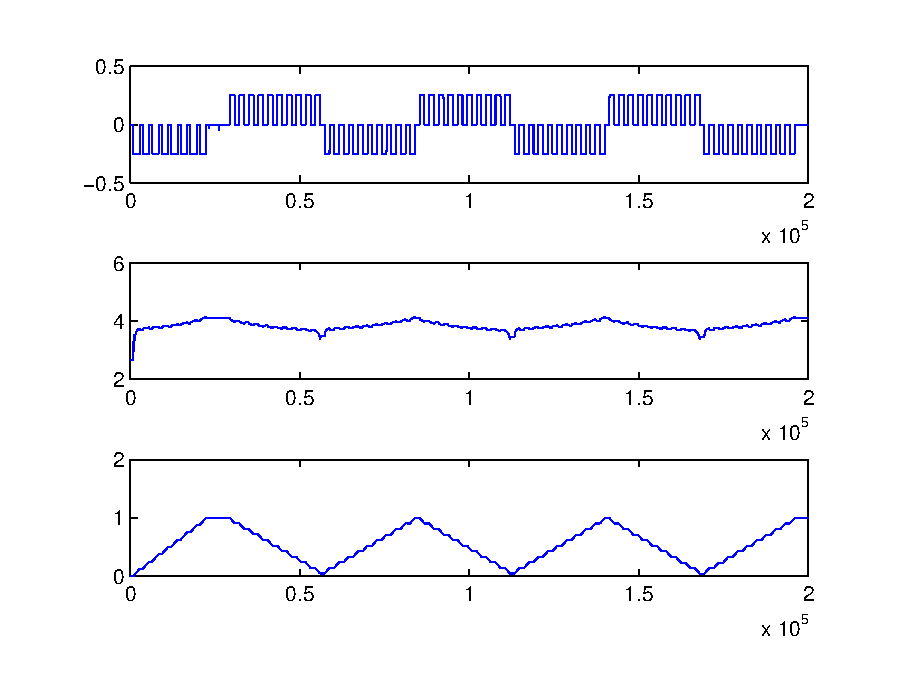
\includegraphics[width=0.9\textwidth]{sim_ideal}
\caption{Discharge current along with the resulting voltage and SOC.}
\label{fig:idealsim}
\end{figure}
